\clearpage
\section{Hardware}\label{sec:Hardware}
Text Robin


\subsection{Bluetooth Mesh Node}\label{subsec:BMN}
Im Bluetooth Mesh Protokoll gibt es zwei verschiedene arten Geräte, in "unprovisioned device" und einen "Node". Das "unprovisioned device" ist ein Teilnehmer, der unbekannt für das Mesh Netzwerk ist und deshalb keine Rechte besitzt. Wird dieses Gerät nun in das Netzwerk aufgenommen, so wird das "unprovisioned device" zu einem Node. Dieses vorgehen nennt sich "provisioning". Die Hardware für den Node besteht bei allen Geräten aus dem gleichen SoC. Der NRF52840 von Nordic Semiconductor eignet sich aus folgenden Gründen perfekt für diese Anwendung. Die Nodes dürfen um eine lange Laufzeit zu generieren, sehr wenig elektrische Leistung beziehen. Der NRF52840 benötigt im Ruhemodus nur wenige micro Ampere. Ein weiterer Grund ist die sehr gute Dokumentation der Software von Nordic Semiconductor. Die gesamte Software ist im Infozenter erhältlich und frei zugänglich. Weitere Forteile befinden sich in der nachfolgenden Tabelle:

% Please add the following required packages to your document preamble:
% \usepackage[normalem]{ulem}
% \useunder{\uline}{\ul}{}
\begin{table}[h]
	\begin{tabular}{ll}
		\multicolumn{2}{l}{{\ul \textbf{Vorteile des nRF52840}}}       \\
		Bluetooth 5                          & -95 dBm Sensivität      \\
		Multiprotokoll (Thread, Zigbee, usw) & +8 dBm Ausgangsleistung \\
		Geringer Stromverbrauch              & USB 2.0                 \\
		12bit ADC                            & NFC                     \\
		1 MB flash und 256kB RAM Speicher    & ARM M4F Cortex         
	\end{tabular}
\end{table}

\begin{figure}[h]
	\centering
	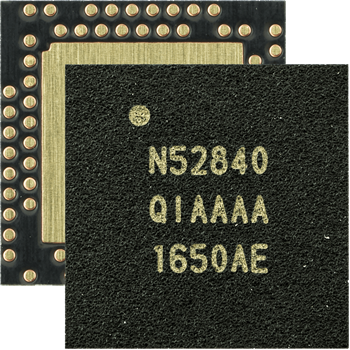
\includegraphics[scale=0.5,angle=0]{nRF52840.png}
	\caption{nRF52840 SoC}
	\label{img:nRF52840}
\end{figure} 


\subsection{Power Management Unit (PMU)}\label{subsec:PMU}